\section{Reconstruction des jets}\label{chapter-JERC-section-jets_reco}
Les particules colorées ne peuvent donc pas être directement observées dans le détecteur.
Leur signature expérimentale est un flux collimé de particules stables composé de hadrons, de leptons et de photons.
La présence de hadrons s'explique directement par le processus de hadronisation décrit dans la section précédente.
Les leptons proviennent de la désintégration, par interaction faible, des hadrons de saveur lourde, ou plus précisément des quarks de deuxième et troisième génération composant ces hadrons lourds.
Les photons sont radiés par les particules électriquement chargées.
\par Un processus physique comme celui de la figure~\ref{subfig-fgraph-Z_q_q} produit seulement quelques particules, en l'occurrence deux, et non des ensembles de particules, comme sur la figure~\ref{fig-agglo_hadronique} qui pourrait correspondre à l'état effectivement observé pour le processus de la figure~\ref{subfig-fgraph-Z_q_q}.
Afin de pouvoir étudier le processus initial, il est nécessaire de définir une observable décrivant les particules colorées à l'origine de ces flux collimés de particules stables.
\par Cette observable est un \og jet \fg.
À partir des particules identifiées à l'aide de l'algorithme de \emph{Particle Flow} (\PF)\footnote{L'algorithme de \emph{Particle Flow} est décrit dans la section~\ifref{chapter-LHC-section-evt_reco-subsec-PF}{\ref{chapter-LHC-section-evt_reco-subsec-PF}}{4.1} du chapitre\ifref{chapter-LHC}{~\ref{chapter-LHC}}{ \og Dispositif expérimental \fg}.}, un algorithme de regroupement permet d'obtenir la liste des jets de l'événement.
Il existe plusieurs algorithmes de regroupement dont le principe est décrit dans la section suivante.
\subsection{Algorithmes de regroupement}\label{chapter-JERC-section-jets_reco-subsec-algo}
Il existe deux catégories d'algorithmes permettant de regrouper les particules en jets, les algorithmes de cônes et les algorithmes de recombinaison séquentielle.
Dans la section~\ref{chapter-JERC-section-jets}, nous avons vu que les radiations de partons sont plus importantes pour de basses énergies (limite infrarouge) ou pour un parton radié colinéaire au parton initial (limite colinéaire).
Afin de conserver des prédictions de QCD vérifiables sur des jets réels, les algorithmes de regroupement doivent être insensibles à l'ajout d'une particule de basse énergie ou au partage d'une particule en deux particules d'énergies inférieures. C'est ce que l'on appelle l'insensibilité IRC, pour \emph{InfraRed and Colinear}.
La plupart des algorithmes de cônes ne sont pas IRC-insensibles, alors que la plupart des algorithmes de recombinaison séquentielle le sont.
\subsubsection{Les algorithmes de cônes}
Les algorithmes de cônes regroupent toutes les particules ayant une direction $\vec{p}$ telle que la distance $\Delta R_{pa}$ à la direction de l'axe du cône $\vec{a}$ dans le plan $(\eta,\phi)$\footnote{Les coordonnées $\eta$ et $\phi$ sont définies dans la section~\ifref{chapter-LHC-section-CMS-subsec-overview_and_coordinates}{\ref{chapter-LHC-section-CMS-subsec-overview_and_coordinates}}{2.1} du chapitre\ifref{chapter-LHC}{~\ref{chapter-LHC}}{ \og Dispositif expérimental \fg}.} est inférieure à une distance de coupure $R_c$, \ie\ si
\begin{equation}
\Delta R_{pa} ^2 = (\eta_p - \eta_a)^2 + (\phi_p - \phi_a)^2 < R_c^2
\mend
\end{equation}
Alors, la direction $\vec{a}$ du cône et redéfinie comme étant la direction moyenne de toutes les particules rassemblées dans ce cône. Ce processus est itéré jusqu'à la stabilisation des cônes.
Enfin, les cônes sont séparés en cas de superposition, une particule ne pouvant appartenir qu'à un seul jet.
\par L'algorithme \textsc{SISCone}~\cite{SISCone}, \emph{Seedless Infrared Safe Cone}, est un exemple d'algorithme de cônes IRC-insensible.
Dans un premier temps, tous les cônes stables possibles sont reconstruits.
Ces cônes sont alors fusionnés, les cônes ayant l'impulsion transverse la plus grande absorbant des cônes d'impulsion transverse moindre dont ils contiennent déjà une fraction.
Un exemple de reconstruction de jets à l'aide de l'algorithme \textsc{SISCone} est présenté sur la figure~\ref{fig-chapter-JERC-section-jets_reco-subsec-algo-examples}.
\subsubsection{Les algorithmes de recombinaison séquentielle}
Les algorithmes de recombinaison séquentielle commencent par considérer que chaque particule forme un jet d'une seule particule.
Puis, à l'aide d'une métrique donnée, la paire de jets les plus proches entre eux fusionne en un seul jet tant que la distance entre eux est en-deçà d'une valeur seuil. Les jets fusionnés donnent la liste des jets de l'événement. Il est également possible de fixer le nombre de jets à déterminer et non la valeur seuil de la distance entre les jets à fusionner.
\par Plusieurs métriques peuvent être définies, chacune correspondant à un algorithme de recombinaison séquentielle proposant des regroupement différents.
\begin{description}
%\item[Algorithme de Durham] La distance $d_{ij}$ entre deux jets $i$ et $j$ est
%\begin{equation}
%d_{ij} = 2 \, \min(E_i^2, E_j^2) \, \frac{1-\cos\theta_{ij}}{Q^2}
%\end{equation}
%où $E_x$ est l'énergie du jet $x$, $\theta_{ij}$ l'angle entre les directions des deux jets et $Q$ l'énergie dans le centre de masse de la collision.
%Cet algorithme a l'avantage de regrouper les particules très fidèlement vis-à-vis de la gerbe hadronique, mais les jets obtenus possèdent une géométrie spatiale irrégulière, comme cela se voit sur la figure~\ref{fig-chapter-JERC-section-jets_reco-subsec-algo-examples}.
\item[Algorithme \kT] La distance $d_{ij}$ entre deux jets $i$ et $j$ est
\begin{equation}
d_{ij} = \min({\pT}_i^2, {\pT}_j^2) \, \frac{\Delta R_{ij}^2}{R^2}
\msep
\Delta R_{ij}^2 = (\eta_i-\eta_j)^2 + (\phi_i-\phi_j)^2
\end{equation}
où ${\pT}_x$ est l'impulsion transverse du jet $x$ et $R$ un paramètre libre.
Cet algorithme a l'avantage de regrouper les particules très fidèlement vis-à-vis de la gerbe hadronique, mais les jets obtenus possèdent une géométrie spatiale irrégulière, comme cela se voit sur la figure~\ref{fig-chapter-JERC-section-jets_reco-subsec-algo-examples}.
\item[Algorithme de Cambridge/Aachen] La distance $d_{ij}$ entre deux jets $i$ et $j$ est
\begin{equation}
d_{ij} = \frac{\Delta R_{ij}^2}{R^2}
\msep
\Delta R_{ij}^2 = (\eta_i-\eta_j)^2 + (\phi_i-\phi_j)^2
\end{equation}
où $R$ est un paramètre libre. Le regroupement des jets est ainsi uniquement basé sur l'écart angulaire.
\item[Algorithme anti-\kT~\cite{Cacciari_antikT}] La distance $d_{ij}$ entre deux jets $i$ et $j$ est
\begin{equation}
d_{ij} = \min\left(\frac{1}{{\pT}_i^2}, \frac{1}{{\pT}_j^2}\right) \, \frac{\Delta R_{ij}^2}{R^2}
\msep
\Delta R_{ij}^2 = (\eta_i-\eta_j)^2 + (\phi_i-\phi_j)^2
\end{equation}
où ${\pT}_x$ est l'impulsion transverse du jet $x$ et $R$ un paramètre libre.
Le regroupement des particules se fait ainsi autour des particules de plus haute énergie.
Cet algorithme propose un regroupement des particules moins fidèle à la gerbe hadronique, mais produit des jets de forme régulière, comme cela se voit sur la figure~\ref{fig-chapter-JERC-section-jets_reco-subsec-algo-examples}.
\end{description}
\begin{figure}[h]
\centering
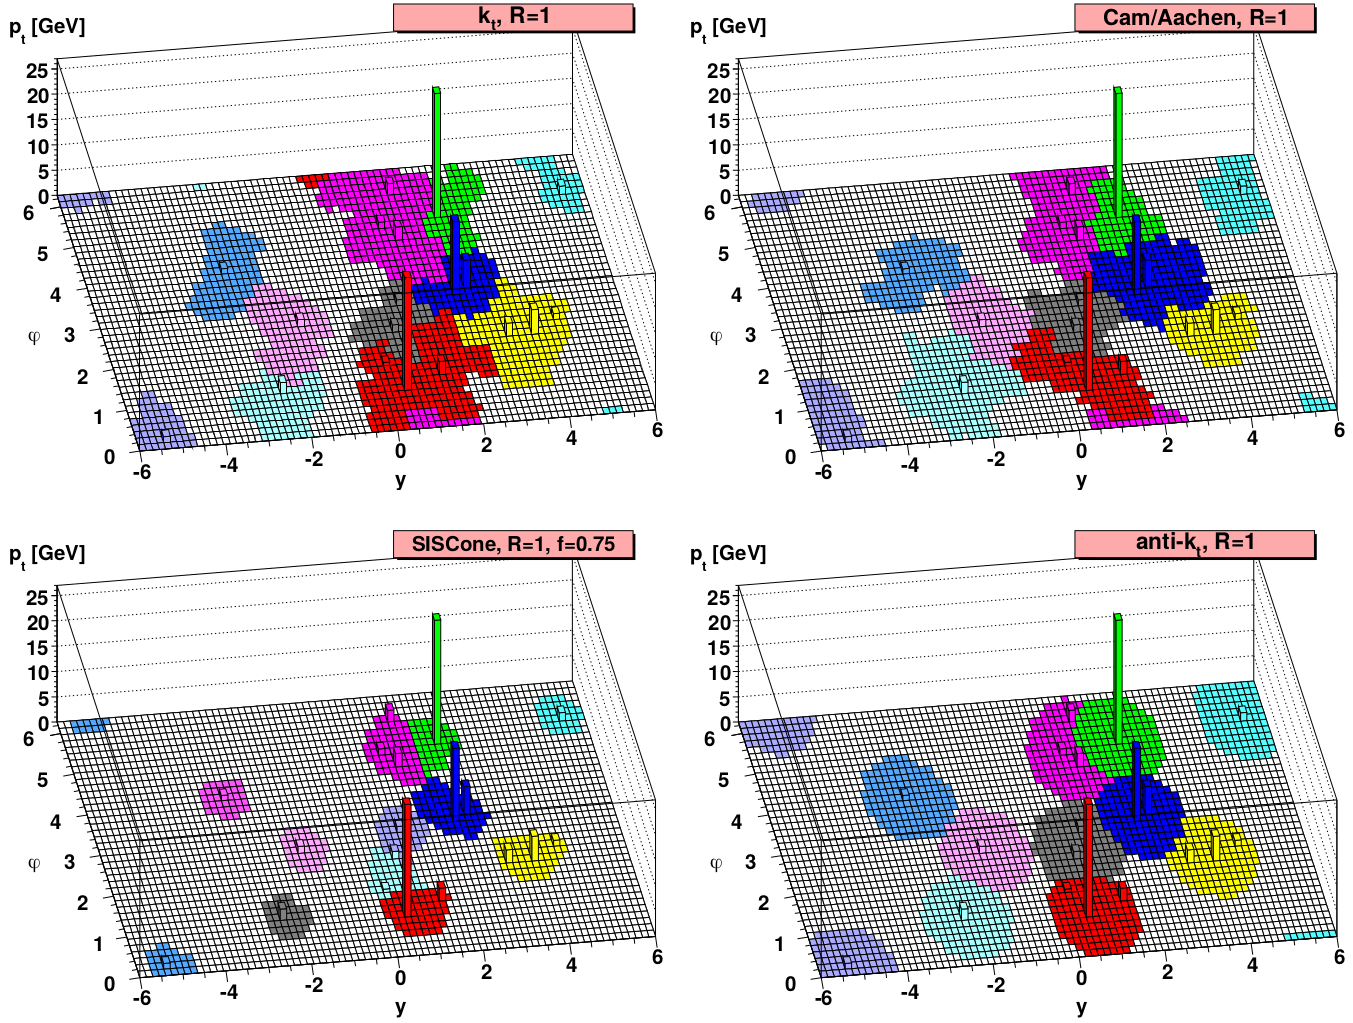
\includegraphics[width=.8\textwidth]{\PhDthesisdir/contents/chapter-JERC/reconstruction_des_jets/forme_des_jets.png}
\caption{Formes des jets reconstruits à partir de différents algorithmes pour un même événement~\cite{Cacciari_antikT}. En haut à gauche, \kT; en haut à droite, C/A; en bas à gauche, \textsc{SISCone}; en bas à droite, anti-\kT. L'algorithme anti-\kT\ permet d'obtenir des jets de forme régulière, conique.}
\label{fig-chapter-JERC-section-jets_reco-subsec-algo-examples}
\end{figure}
\par Le temps de calcul de ces algorithmes est un enjeu majeur au LHC.
Leurs temps d'exécution sont représentés en fonction du nombre d'événements d'empilement sur la figure~\ref{fig-chapter-JERC-section-jets_reco-subsec-algo-perfs}.
L'algorithme anti-\kT\ se place parmi les algorithmes les plus rapides.
Dans les conditions des collisions proton-proton du LHC, il permet le traitement d'un événement en moins d'une milliseconde.
C'est cet algorithme de regroupement qui est utilisé dans le cadre de l'expérience CMS.
\begin{figure}[h]
\centering
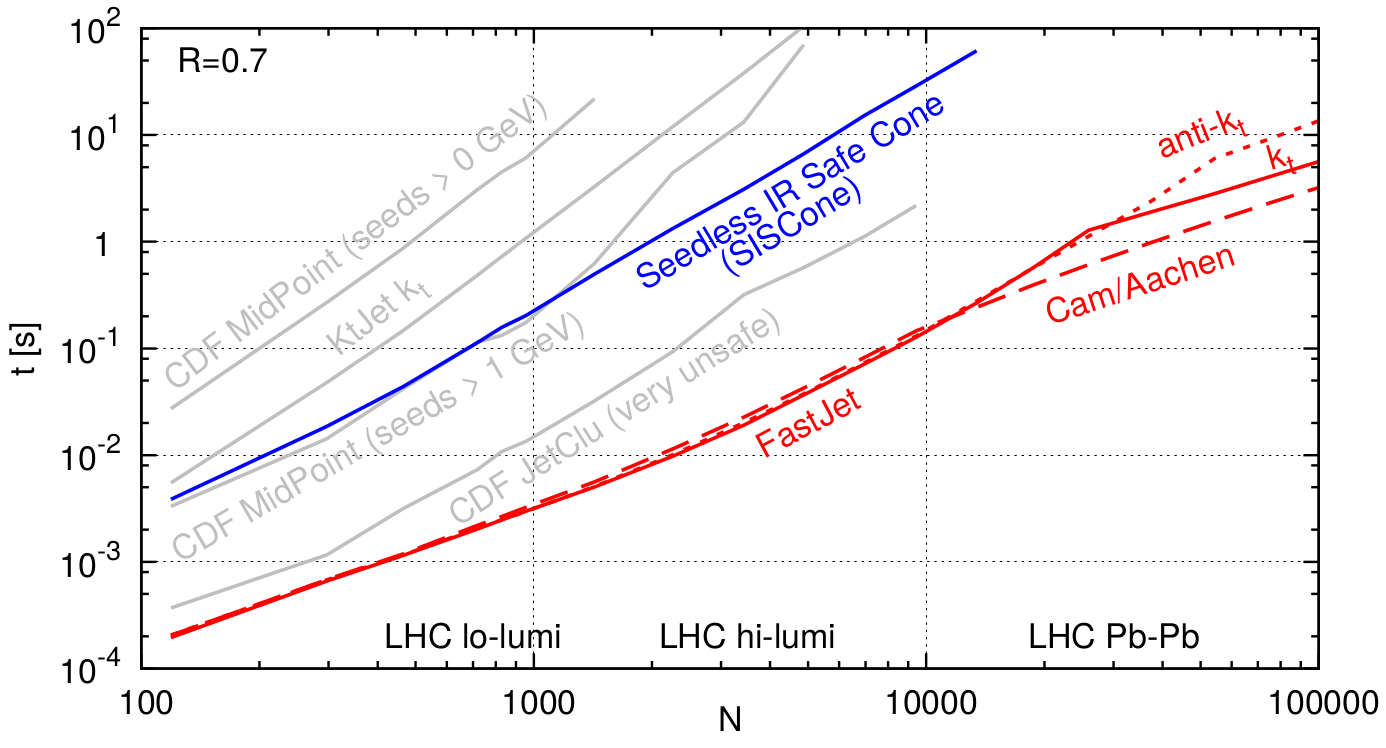
\includegraphics[width=.6\textwidth]{\PhDthesisdir/contents/chapter-JERC/reconstruction_des_jets/temps_de_calcul.png}
\caption{Temps de reconstruction d'un empilement d'un événement di-jets avec $N$ événements ne produisant que des jets de bas \pT\ pour différents algorithmes de reconstruction des jets.} % 50 GeV
\label{fig-chapter-JERC-section-jets_reco-subsec-algo-perfs}
\end{figure}
\subsection{Identification des jets dans CMS}\label{chapter-JERC-section-jets_reco-subsec-jetID}
Les jets ainsi reconstruits à l'aide des algorithmes de recombinaison sont en fait des \og candidats \fg{} jets.
À l'instar des particules individuelles, des critères d'identification leur sont appliqués afin de rejeter le bruit de fond et s'assurer de la qualité des jets ainsi reconstruits.
\par Ces critères reposent sur les caractéristiques des candidats jets comme la fraction d'énergie provenant de leurs constituants neutres ou encore le nombre de ces constituants.
Ces critères dépendent des années de prise de données et de la pseudo-rapidité du jet, \ie\ de la région du détecteur dans laquelle il se trouve.
\par Les critères utilisés pour les années 2016, 2017 et 2018, listés page~\pageref{tab-chapter-JERC-section-jets_reco-subsec-jetID-2017UL}, permettent d'obtenir une efficacité d'identification des jets supérieure à \SI{99}{\%} dans chacune des régions en $\eta$ du détecteur.
La réjection du bruit de fond est supérieure à \SI{98}{\%} pour $\abs{\eta}\leq\num{3.0}$ et supérieure à \SI{36}{\%} pour $\abs{\eta}>\num{3.0}$.
\begin{table}[p]
\centering
\begin{tabularx}{\textwidth}{lcYcY}
\toprule
Propriété du jet à identifier & $\abs{\eta}\leq\num{2.4}$ & $\num{2.4}<\abs{\eta}\leq\num{2.7}$ & $\num{2.7}<\abs{\eta}\leq\num{3.0}$ & $\num{3.0}<\abs{\eta}$ \\
\midrule
Fraction d'énergie\\
\labelitemi\ hadronique neutre & $<\num{0.90}$ & $<\num{0.90}$ & $<\num{0.98}$ & \\
\labelitemi\ électromagnétique neutre & $<\num{0.90}$ & $<\num{0.90}$ & $>\num{0.01}$ & $<\num{0.90}$ \\
\labelitemi\ hadronique chargée & $>\num{0}$ &&&\\
\labelitemi\ électromagnétique chargée & $<\num{0.99}$ &&&\\
\midrule
Nombre de constituants\\
\labelitemi\ neutres & $>\num{1}$ & $>\num{1}$ & $>\num{2}$ & $>\num{10}$ \\
\labelitemi\ chargés & $>\num{0}$ &&&\\
\bottomrule
\end{tabularx}

\caption{Critères d'identification des jets à CMS pour l'analyse des données de 2016.}
\label{tab-chapter-JERC-section-jets_reco-subsec-jetID-2016}
\end{table}
\begin{table}[p]
\centering
\begin{tabularx}{\textwidth}{lcYcY}
\toprule
Propriété du jet à identifier & $\abs{\eta}\leq\num{2.4}$ & $\num{2.4}<\abs{\eta}\leq\num{2.7}$ & $\num{2.7}<\abs{\eta}\leq\num{3.0}$ & $\num{3.0}<\abs{\eta}$ \\
\midrule
Fraction d'énergie\\
\labelitemi\ hadronique neutre & $<\num{0.90}$ & $<\num{0.90}$ &  & $>\num{0.02}$ \\
\labelitemi\ électromagnétique neutre & $<\num{0.90}$ & $<\num{0.90}$ & $<\num{0.99}$ et $>\num{0.02}$ & $<\num{0.90}$ \\
\labelitemi\ hadronique chargée & $>\num{0}$ &&&\\
\labelitemi\ électromagnétique chargée & $<\num{0.8}$ \\
\labelitemi\ muonique & $<\num{0.8}$ & $<\num{0.8}$ \\
\midrule
Nombre de constituants & $>\num{1}$ & $>\num{1}$\\
\labelitemi\ neutres & & & $>\num{2}$ & $>\num{10}$ \\
\labelitemi\ chargés & $>\num{0}$ &&&\\
\bottomrule
\end{tabularx}

\caption{Critères d'identification des jets à CMS pour l'analyse des données de 2017.}
\label{tab-chapter-JERC-section-jets_reco-subsec-jetID-2017}
\end{table}
\begin{table}[p]
\centering
\begin{tabularx}{\textwidth}{lcYcY}
\toprule
Propriété du jet à identifier & $\abs{\eta}\leq\num{2.6}$ & $\num{2.6}<\abs{\eta}\leq\num{2.7}$ & $\num{2.7}<\abs{\eta}\leq\num{3.0}$ & $\num{3.0}<\abs{\eta}\leq\num{5.0}$ \\
\midrule
Fraction d'énergie\\
\labelitemi\ hadronique neutre & $<\num{0.90}$ & $<\num{0.90}$ &  & $>\num{0.2}$ \\
\labelitemi\ électromagnétique neutre & $<\num{0.90}$ & $<\num{0.99}$ & $<\num{0.99}$ et $>\num{0.02}$ & $<\num{0.90}$ \\
\labelitemi\ hadronique chargée & $>\num{0}$ &&&\\
\midrule
Nombre de constituants & $>\num{1}$\\
\labelitemi\ neutres & & & $>\num{2}$ & $>\num{10}$ \\
\labelitemi\ chargés & $>\num{0}$ & $>\num{0}$ &&\\
\bottomrule
\end{tabularx}

\caption{Critères d'identification des jets à CMS pour l'analyse des données de 2018.}
\label{tab-chapter-JERC-section-jets_reco-subsec-jetID-2018}
\end{table}
\begin{table}[p]
\centering
\begin{tabularx}{\textwidth}{lcYcY}
\toprule
Propriété du jet à identifier & $\abs{\eta}\leq\num{2.6}$ & $\num{2.6}<\abs{\eta}\leq\num{2.7}$ & $\num{2.7}<\abs{\eta}\leq\num{3.0}$ & $\num{3.0}<\abs{\eta}\leq\num{5.0}$ \\
\midrule
Fraction d'énergie\\
\labelitemi\ hadronique neutre & $<\num{0.90}$ & $<\num{0.90}$ &  & $>\num{0.2}$ \\
\labelitemi\ électromagnétique neutre & $<\num{0.90}$ & $<\num{0.99}$ & $<\num{0.99}$ et $>\num{0.01}$ & $<\num{0.90}$ \\
\labelitemi\ hadronique chargée & $>\num{0}$ &&&\\
\labelitemi\ électromagnétique chargée & $<\num{0.8}$ & $<\num{0.8}$ \\
\labelitemi\ muonique & $<\num{0.8}$ & $<\num{0.8}$ \\
\midrule
Nombre de constituants & $>\num{1}$\\
\labelitemi\ neutres & & & $>\num{1}$ & $>\num{10}$ \\
\labelitemi\ chargés & $>\num{0}$ & $>\num{0}$ &&\\
\bottomrule
\end{tabularx}

\caption{Critères d'identification des jets à CMS pour l'analyse des données de 2017-UL.}
\label{tab-chapter-JERC-section-jets_reco-subsec-jetID-2017UL}
\end{table}
\subsection{Saveur des jets}\label{chapter-JERC-section-jets_reco-subsec-flavor}
Pour étudier la physique du processus initial, la connaissance de la particule colorée à l'origine d'un jet ainsi identifié dans le détecteur est une information de choix.
Il est impossible de connaître avec certitude cette particule, mais sa nature influe directement sur certaines propriétés des jets, permettant de l'estimer.
\subsubsection{Saveur de la particule initiale et caractéristiques des jets}
\paragraph{Le quark~\quarkt} possède un temps de vie trop court pour participer à l'hadronisation. Il se désintègre alors par interaction faible en un autre quark, très majoritairement un quark~\quarkb, et un boson \Wboson. Le nouveau quark issu de cette désintégration forme alors un jet.
\par Les autres quarks, \quarkd, \quarku, \quarks, \quarkc\ et~\quarkb, sont plus stables que le top et participent à l'hadronisation.
Ils se retrouvent alors confinés au sein des hadrons formés.
\paragraph{Le quark~\quarkb} ne forme pas de hadron stable. Il se désintègre en quark~\quarkc\ ou~\quarku\ selon
\begin{equation}
\quarkb \to \quarkc\Wbosonminus
\msep
\antiquarkb \to \antiquarkc\Wbosonplus
\msep
\quarkb \to \quarku\Wbosonminus
\msep
\antiquarkb \to \antiquarku\Wbosonplus
\mend
\end{equation}
Ces désintégrations font intervenir les modules des coefficients $V_{\quarkc\quarkb}$ et $V_{\quarku\quarkb}$ de la matrice CKM\footnote{La matrice CKM est introduite dans la section~\ifref{chapter-MS-MSSM-section-formalisme-subsec-EW-quarks}{\ref{chapter-MS-MSSM-section-formalisme-subsec-EW-quarks}}{2.3.4} du chapitre\ifref{chapter-MS-MSSM}{~\ref{chapter-MS-MSSM}}{ \og Particules, interactions et phénoménologie \fg}.} dont les valeurs sont faibles et sont donc fortement supprimées.
\par Les hadrons contenant un quark~\quarkb\ ont ainsi une durée de vie $\tau$ de l'ordre de la picoseconde~\cite{B0s_lifetime,lifetimes_c_b_hadrons} et peuvent voyager sur une distance de l'ordre du millimètre.
Les traces des particules chargées issues de cette nouvelle désintégration proviennent donc d'un vertex secondaire (SV), différent du vertex primaire (PV).
Ces traces sont \og déplacées \fg.
Pour chacune d'entre elles, il est possible de déterminer le paramètre d'impact (IP) au vertex primaire, dont la valeur est typiquement plus grande que pour des traces provenant du vertex primaire, comme cela est illustré sur la figure~\ref{fig-chapter-JERC-section-jets_reco-subsec-flavor-SV_scheme}.
\begin{figure}[h]
\centering
\begin{tikzpicture}[scale=1.5]
\def\trackerrin{.100}
\def\trackerrout{1.185}
\def\trackercolor{ltcolorgray1}

\def\ECALrin{1.290}
\def\ECALrout{1.811}
\def\ECALcolor{ltcolorgreen1}

\def\HCALrin{1.812}
\def\HCALrout{2.854}
\def\HCALcolor{ltcoloryellow3}

\def\Solenrin{2.950}
\def\Solenrout{3.800}
\def\Solencolor{ltcolorgray2}

\def\ironryrina{3.850}
\def\ironryrouta{4.000}
\def\muonrina{4.020}
\def\muonrouta{4.400}
\def\ironryrinb{4.420}
\def\ironryroutb{4.880}
\def\muonrinb{4.905}
\def\muonroutb{5.285}
\def\ironryrinc{5.300}
\def\ironryroutc{5.960}
\def\muonrinc{5.975}
\def\muonroutc{6.355}
\def\ironryrind{6.375}
\def\ironryroutd{6.980}
\def\muonrind{7.000}
\def\muonroutd{7.380}
\def\muoncolor{ltcoloryellow1}
\def\ironrycolor{ltcolorred2}

\def\printele#1{
\draw [thick, ltcolorred] (0,0) arc (#1-90:#1-90+27:3) coordinate (eledeposit);
\draw [ltcolorred] (#1-5:1.25) node {\ele};
}
\def\printmu#1{
\draw [thick, ltcolorblue] (0,0) arc (#1-90:#1-90+33:6) arc (#1-90+33:#1-90:-12) node{\mu};
\draw [ltcolorblue] (#1-7:1.5) node {\mu};
}

\def\printantiele#1{
\draw [thick, ltcolorred] (0,0) arc (#1-90:#1-90-27:-3) coordinate (eledeposit);
\draw [ltcolorred] (#1-7:1.5) node {\ele};
%\draw [ltcolorred4, ultra thick] (eledeposit)--+(#1+25:\ECALrout);
}
\def\printantimu#1{
\draw [thick, ltcolorblue] (0,0) arc (#1-90:#1-90-33:-6) arc (#1-90-33:#1-90:12);
\draw [ltcolorblue] (#1-7:1.5) node {\mu};
}

\def\printtauh#1{
\draw [thick, ltcolorgreen4] (0,0) arc (#1-90:#1-90+11:10) ;
\draw [thick, ltcolorgreen4] (0,0) arc (#1-90:#1-90+6:20) ;
\draw [thick, ltcolorgreen4] (0,0) arc (#1-90:#1-90-11:-10) ;
\draw [ltcolorgreen4] (#1-12:1.5) node {\tauh};
}
\def\printantitauh#1{
\draw [thick, ltcolorgreen4] (0,0) arc (#1-90:#1-90-11:-10) ;
\draw [thick, ltcolorgreen4] (0,0) arc (#1-90:#1-90-6:-20) ;
\draw [thick, ltcolorgreen4] (0,0) arc (#1-90:#1-90+11:10) ;
\draw [ltcolorgreen4] (#1-12:1.5) node {\tauh};
}

\def\printjetnolabel#1{
\draw [thick, ltcolororange] (0,0) arc (#1-90+10:#1-90+22+10:5) ;
\draw [thick, ltcolororange] (0,0) arc (#1-90+5:#1-90+12+5:10) ;
\draw [thick, ltcolororange] (0,0) arc (#1-90:#1-90-22:-5) ;
\draw [thick, ltcolororange] (0,0) arc (#1-90:#1-90+6:20) ;
\draw [thick, ltcolororange] (0,0) arc (#1-90+5:#1-90+8+5:10) ;
\draw [thick, ltcolororange] (0,0) arc (#1-90:#1-90-11:-10) ;
\draw [thick, ltcolororange] (0,0) arc (#1-90:#1-90+11:10) ;
}

\def\printjet#1{
\printjetnolabel{#1}
\draw [ltcolororange] (#1-25:.5) node {jet};
}

\def\printjetfake#1{
\printjet{#1}
\draw [thick, ltcolorgreen4] (0,0) arc (#1-90:#1-90+11:10) ;
\draw [thick, ltcolorgreen4] (0,0) arc (#1-90:#1-90+6:20) ;
\draw [thick, ltcolorgreen4] (0,0) arc (#1-90:#1-90-11:-10) ;
\draw [ltcolorgreen4] (#1-17:1.5) node {f.\tauh};
}

\def\printdeposit#1#2#3#4{
\fill [#1] (#2-2:#3) arc (#2-2:#2+2:#3) -- (#2+2:#4) arc (#2+2:#2-2:#4) ;
}

\def\printECALdeposit#1#2{\printdeposit{#1}{#2}{\ECALrin}{\ECALrout}}
\def\printHCALdeposit#1#2{\printdeposit{#1}{#2}{\HCALrin}{\HCALrout}}

\def\printtauhdeposit#1{
\printHCALdeposit{ltcoloryellow4}{#1+3}
\printHCALdeposit{ltcoloryellow4}{#1+5}
\printHCALdeposit{ltcoloryellow4}{#1-5}
}

\def\printjetdeposit#1{
\printHCALdeposit{ltcoloryellow4}{#1+3}
\printHCALdeposit{ltcoloryellow4}{#1+5}
\printHCALdeposit{ltcoloryellow4}{#1-5}
\printHCALdeposit{ltcoloryellow4}{#1+21}
\printHCALdeposit{ltcoloryellow4}{#1+11}
\printHCALdeposit{ltcoloryellow4}{#1-11}
}

\def\printMuChSigA#1#2{
\fill [red] (#1-7.5+20*#2:\muonrina) arc (#1-7.5+20*#2:#1+7.5+20*#2:\muonrina) -- (#1+7.5+20*#2:\muonrouta) arc (#1+7.5+20*#2:#1-7.5+20*#2:\muonrouta) ;
}
\def\printMuChSigB#1#2{
\fill [red] (#1-7.5+20*#2:\muonrinb) arc (#1-7.5+20*#2:#1+7.5+20*#2:\muonrinb) -- (#1+7.5+20*#2:\muonroutb) arc (#1+7.5+20*#2:#1-7.5+20*#2:\muonroutb) ;
}
\def\printMuChSigC#1#2{
\fill [red] (#1-7.5+20*#2:\muonrinc) arc (#1-7.5+20*#2:#1+7.5+20*#2:\muonrinc) -- (#1+7.5+20*#2:\muonroutc) arc (#1+7.5+20*#2:#1-7.5+20*#2:\muonroutc) ;
}
\def\printMuChSigD#1#2{
\fill [red] (#1-7.5+20*#2:\muonrind) arc (#1-7.5+20*#2:#1+7.5+20*#2:\muonrind) -- (#1+7.5+20*#2:\muonroutd) arc (#1+7.5+20*#2:#1-7.5+20*#2:\muonroutd) ;
}

\def\Bjetangle{30}
\def\Bhaddronangle{5}
\def\Bhaddronflight{.75}

\clip (-145:\Solenrin) rectangle (\Bjetangle:1.8*\Solenrin);

\foreach\jetangle in {120,-145}{
\printbigjetnolabel{\jetangle}
\draw (\jetangle:2.5) node {jet} ;
}

\def\CurrentVertex{(\Bhaddronangle:\Bhaddronflight)}

\draw [thick, dotted] (0,0) -- \CurrentVertex ;

{
\def\jetcolor{ltcolorred}
\printjetnolabel{\Bjetangle}
\draw [\jetcolor] (\Bjetangle:2)+(1.5,.75) node {traces déplacées};
}
\begin{scope}
\clip circle (\Solenrin);
\printantimuonnolabel{\Bjetangle}
\end{scope}

\draw [\muoncolor] (\Bjetangle:4) +(0,{-2*\baselineskip}) node {lepton chargé};

\draw (\Bjetangle:4) + (-.125,-.5) circle (1.125);
\draw [-latex] (\Bjetangle:4) + (-.125,-1.625) --+ (-.125,-2) node [below] {jet de saveur lourde};

\draw (0,0) node [left] {PV} ;
\draw \CurrentVertex node [below right] {SV} ;

\fill (0,0) circle (2pt);
\fill \CurrentVertex circle (2pt);

\draw [dashed] \CurrentVertex --+ (\Bjetangle:-.8);

\draw [red, latex-latex] (0,0)--+ (-90+\Bjetangle:{\Bhaddronflight*sin(\Bjetangle-\Bhaddronangle)}) node [below right] {IP};
\end{tikzpicture}
\caption{Illustration d'un jet de saveur lourde. Les particules composant ce jet proviennent d'un vertex secondaire (SV), différent du vertex primaire (PV) où a lieu la collision entre les protons et la formation du hadron lourd à l'origine du SV. Le paramètre d'impact (IP) est également indiqué.}
\label{fig-chapter-JERC-section-jets_reco-subsec-flavor-SV_scheme}
\end{figure}
\par Le boson \Wboson\ issu du changement de saveur du quark~\quarkb\ se désintègre leptoniquement dans \SI{30}{\%} des cas~\cite{PDG_booklet_2018} selon
\begin{equation}
\Wbosonpm \to \ell^\pm \nu_\ell
\mend
\end{equation}
Le lepton chargé donne une signature caractéristique lors des collisions proton-proton ayant lieu au LHC. Dans les autres cas, le \Wboson\ se désintègre hadroniquement selon
\begin{equation}
\Wbosonpm \to \quark\antiquark
\mend
\end{equation}
Le nombre de constituants du jet, ainsi que le nombre de traces déplacées, est alors plus important.
\paragraph{Le quark~\quarkc} suit le même schéma que le quark~\quarkb. Cependant, son canal de désintégration principal est
\begin{equation}
\quarkc \to \quarks\Wbosonplus
\msep
\antiquarkc \to \antiquarks\Wbosonminus
\mend[,]
\end{equation}
ce qui fait intervenir le module du coefficient $V_{\quarkc\quarks}$ de la matrice CKM, proche de 1.
Les hadrons contenant un quark~\quarkc\ ont ainsi une durée de vie $\tau$ de inférieure à la picoseconde~\cite{lifetimes_c_b_hadrons} et il est plus difficile d'identifier les jets issus de quarks~\quarkc\ que ceux issus de quarks~\quarkb.
\paragraph{Les quarks~\quarkd, \quarku\ et~\quarks} forment des hadrons étant:
\begin{itemize}
\item très instables, par exemple les \pionnull, dont seuls les produits de désintégration sont observés;
\item faiblement instables, par exemple les \Kaonplus, qui peuvent se propager jusque dans les parties sensibles du détecteur et donc être directement observés;
\item stables, par exemple les protons, qui sont directement observés dans le détecteur.
\end{itemize}
Dans tous les cas, les traces des particules chargées observées proviennent du PV, lieu de formation du quark initial.
Le phénomène décrit précédemment pour les quarks~\quarkb\ et~\quarkc\ n'est donc pas observable.
Les jets issus de ces trois types de quarks, les plus légers, sont ainsi regroupés sous la dénomination de \og jets légers \fg.
\paragraph{Les gluons} portent une charge de couleur plus importante que les quarks\footnote{Les quarks portent une couleur, les antiquarks une anticouleur et les gluons portent une couleur et une anticouleur.}.
Les jets initiés par des gluons comportement typiquement plus de particules électriquement chargées et sont moins collimés que les jets légers~\cite{CMS-PAS-JME-13-002}.
\subsubsection{Identification de la saveur des jets}
Les jets présentent ainsi des propriétés caractéristiques, selon qu'il s'agisse d'un jet léger (quarks~\quarkd, \quarku\ ou~\quarks), d'un jet lourd (quarks~\quarkc\ ou~\quarkb) ou d'un jet issu d'un gluon.
En utilisant ces propriétés, des algorithmes d'identification de la saveur des jets ont été mis au point par la collaboration CMS~\cite{jet_btag_CSV_RunI}.
Les avancées récentes dans le domaine du \emph{Deep Learning}, appliquées à l'identification des jets~\cite{jet_flavor_deep_nn}, ont permis l'amélioration de ces algorithmes. L'algorithme \DeepCSV~\cite{Sirunyan_heavy_flavor_jets_2018} a ainsi été développé.
\par Les variables utilisées dans cet algorithme sont décrites dans la référence~\cite{Sirunyan_heavy_flavor_jets_2018}.
Elles sont traitées par un réseau de neurones profond de quatre couches cachées de 100 nœuds connectés les uns aux autres.
Ce réseau est entraîné sur un ensemble d'événements simulés $\quarkt\antiquarkt$, présentant de nombreux jets de quarks~\quarkb, et multi-jets à l'aide des librairies
\KERAS~\cite{keras}
et
\TENSORFLOW~\cite{tensorflow}.
\par Les performances ainsi obtenues pour l'algorithme \DeepCSV\ peuvent sont comparées à d'autres algorithme d'identification de la saveur des jets sur la figure~\ref{fig-chapter-JERC-section-jets_reco-subsec-flavor-bc_tag_roc_curves}.
Les algorithmes \textsc{cMVAv2} et \DeepCSV\ présentent les meilleures performances en termes d'identification des jets de quark~\quarkb.
Pour le traitement des jets de quark~\quarkc, l'algorithme \DeepCSV\ propose les meilleures performances.
Dans les analyses présentées dans ce chapitre et le chapitre\ifref{chapter-HTT_analysis}{~\ref{chapter-HTT_analysis}}{~5}, c'est cet algorithme qui est utilisé afin d'identifier les jets issus de quarks~\quarkc\ ou~\quarkb.
\begin{figure}[h]
\centering

\subcaptionbox{Probabilité de mauvaise identification en tant que jet de quark~\quarkb\ de jets de gluon ou quarks légers (traits pleins) ou de jets de quark~\quarkc\ (pointillés) en fonction de l'efficacité d'identification des jets de quark~\quarkb.\label{subfig-chapter-JERC-section-jets_reco-subsec-flavor-b_or_mis}}[.75\textwidth]
{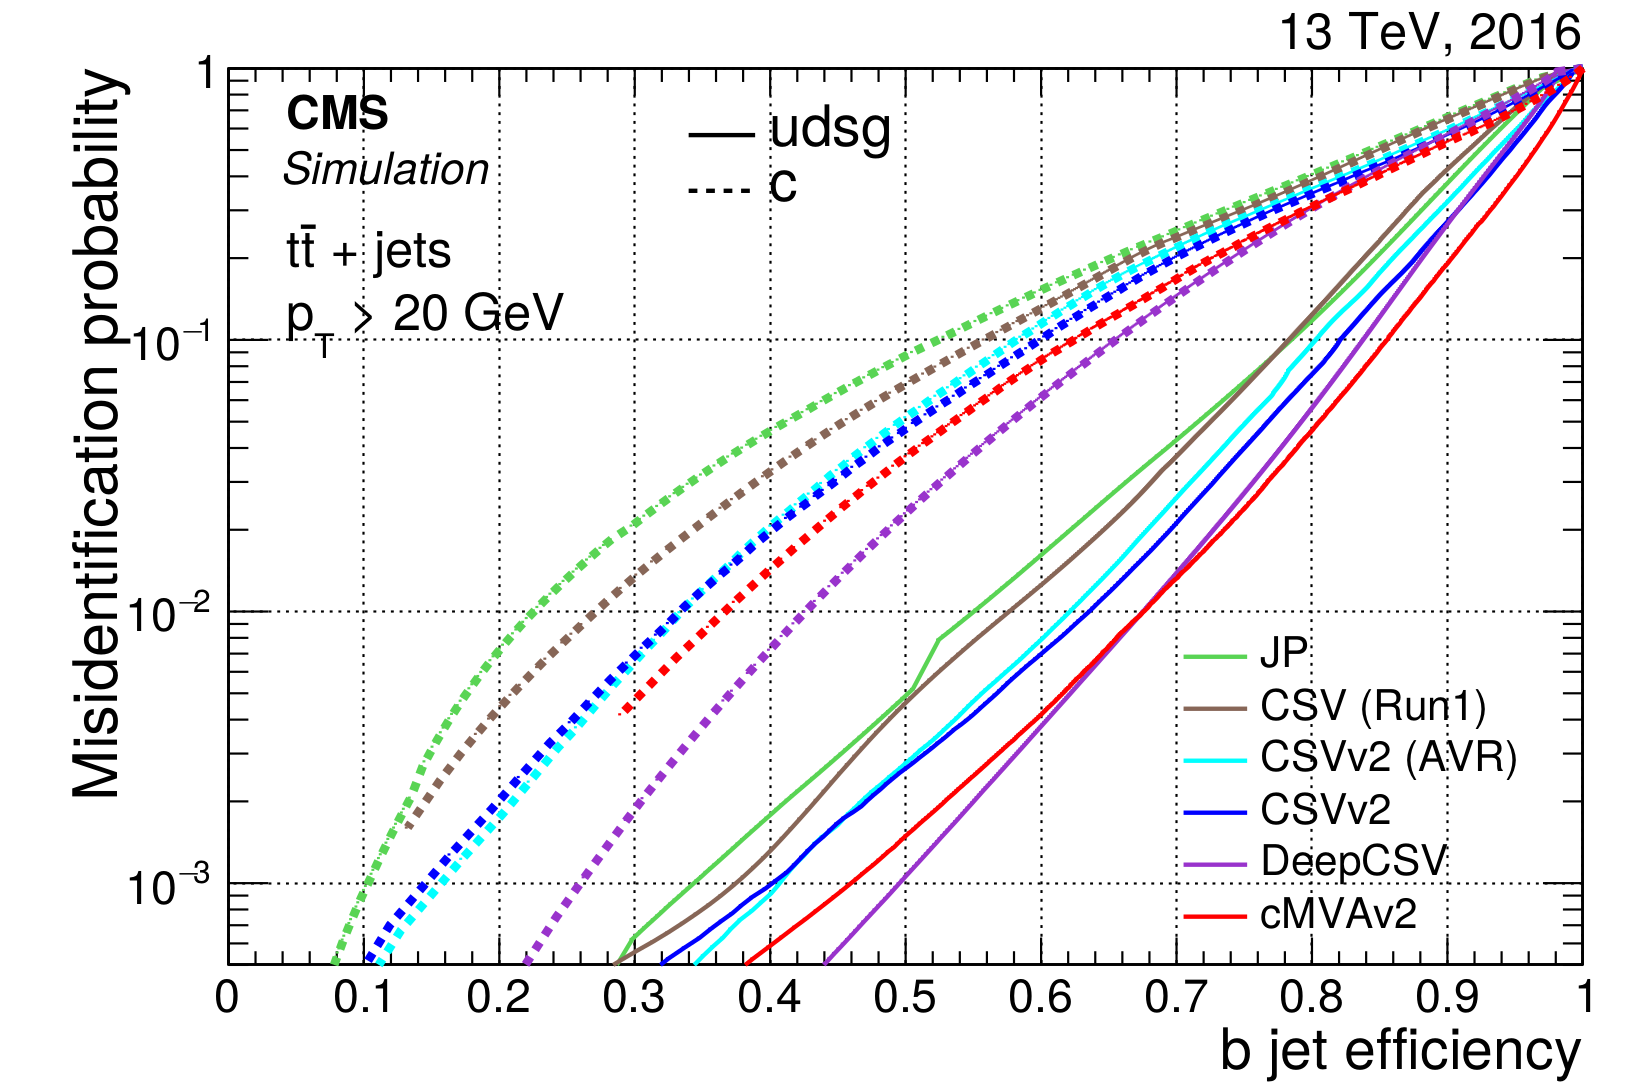
\includegraphics[width=.45\linewidth]{\PhDthesisdir/contents/chapter-JERC/reconstruction_des_jets/Btag_roc_curves/b_or_mis.png}}

\vspace{\baselineskip}

\subcaptionbox{Probabilité de mauvaise identification en tant que jet de quark~\quarkc\ de jets de gluon ou quarks légers en fonction de l'efficacité d'identification des jets de quark~\quarkc.\label{subfig-chapter-JERC-section-jets_reco-subsec-flavor-c_or_mis}}[.45\textwidth]
{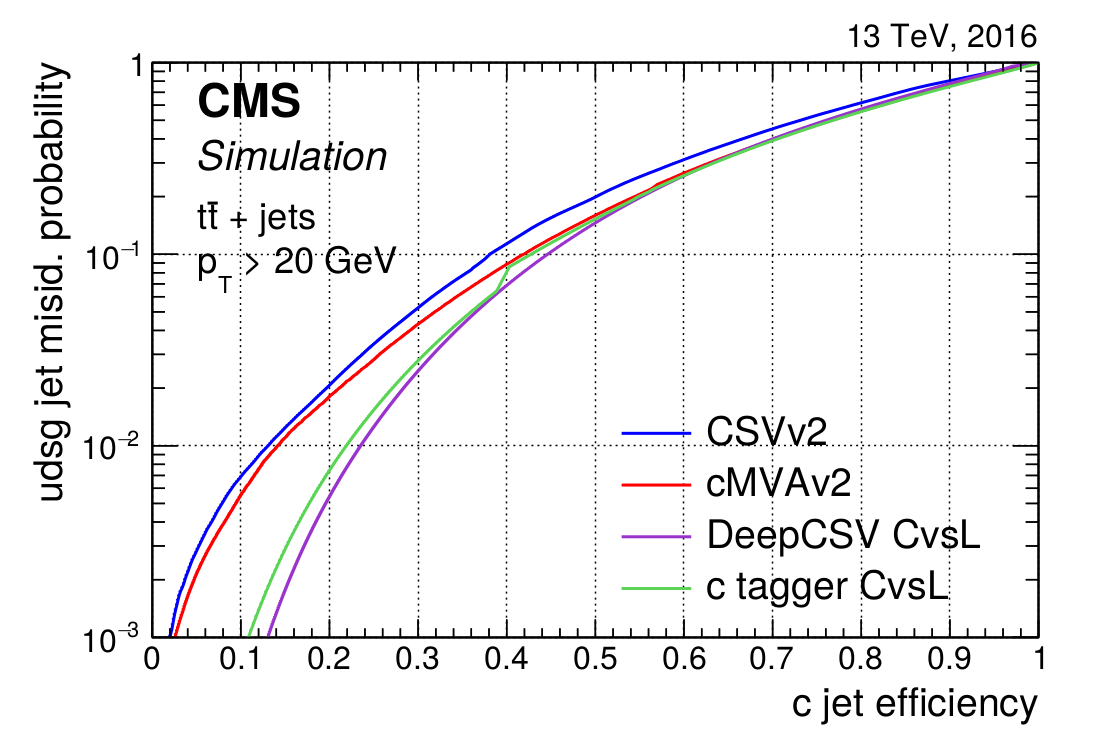
\includegraphics[width=.45\linewidth]{\PhDthesisdir/contents/chapter-JERC/reconstruction_des_jets/Btag_roc_curves/c_or_mis.png}}
\hfill
\subcaptionbox{Probabilité de mauvaise identification en tant que jet de quark~\quarkb\ de jets de quark~\quarkc en fonction de l'efficacité d'identification des jets de quark~\quarkc.\label{subfig-chapter-JERC-section-jets_reco-subsec-flavor-c_or_b}}[.45\textwidth]
{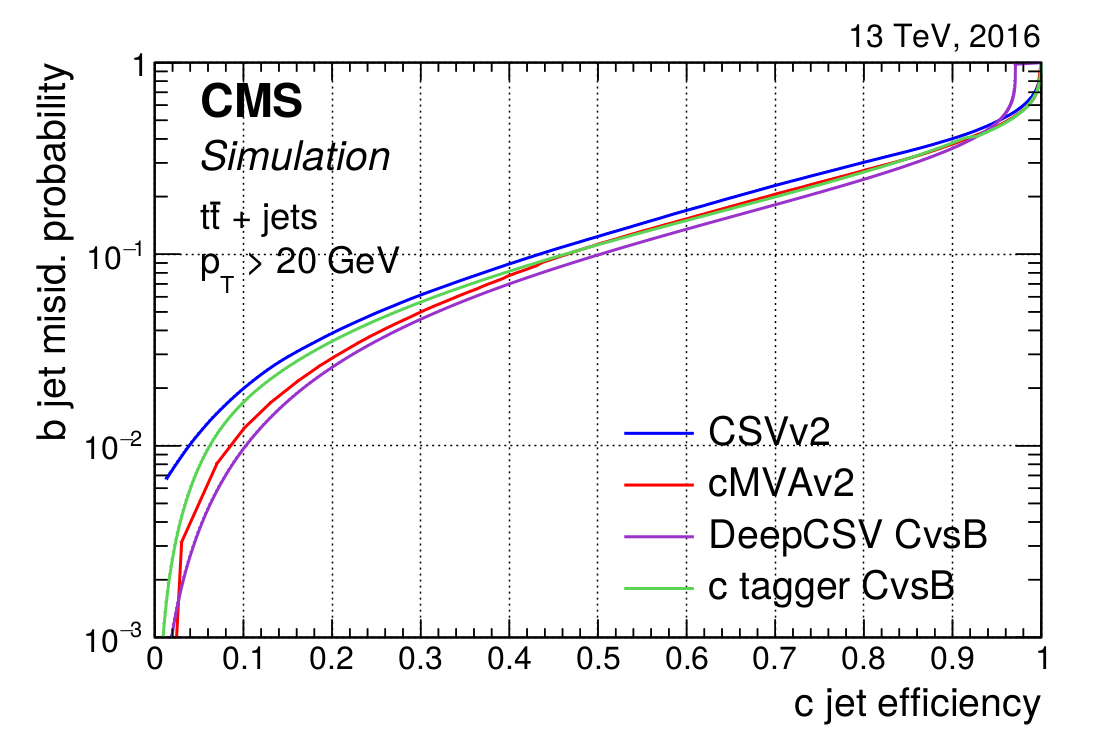
\includegraphics[width=.45\linewidth]{\PhDthesisdir/contents/chapter-JERC/reconstruction_des_jets/Btag_roc_curves/c_or_b.png}}

\caption{Comparaison des performances des algorithmes d'identification de la saveur des jets~\cite{Sirunyan_heavy_flavor_jets_2018}.}
\label{fig-chapter-JERC-section-jets_reco-subsec-flavor-bc_tag_roc_curves}
\end{figure}
\par La discrimination entre jet léger et jet initié par un gluon peut être réalisée à l'aide d'une fonction de vraisemblance~\cite{CMS-PAS-JME-13-002} renvoyant un score entre 0 et 1 pour chaque jet, correspondant à la probabilité que ce jet soit issu d'un quark. La densité de probabilité de cette fonction, selon qu'il s'agisse de jets initiés par des gluons ou des quarks, est représentée sur la figure~\ref{fig-chapter-JERC-section-jets_reco-subsec-flavor-qgl_likelihood}.
\begin{figure}[h]
\centering
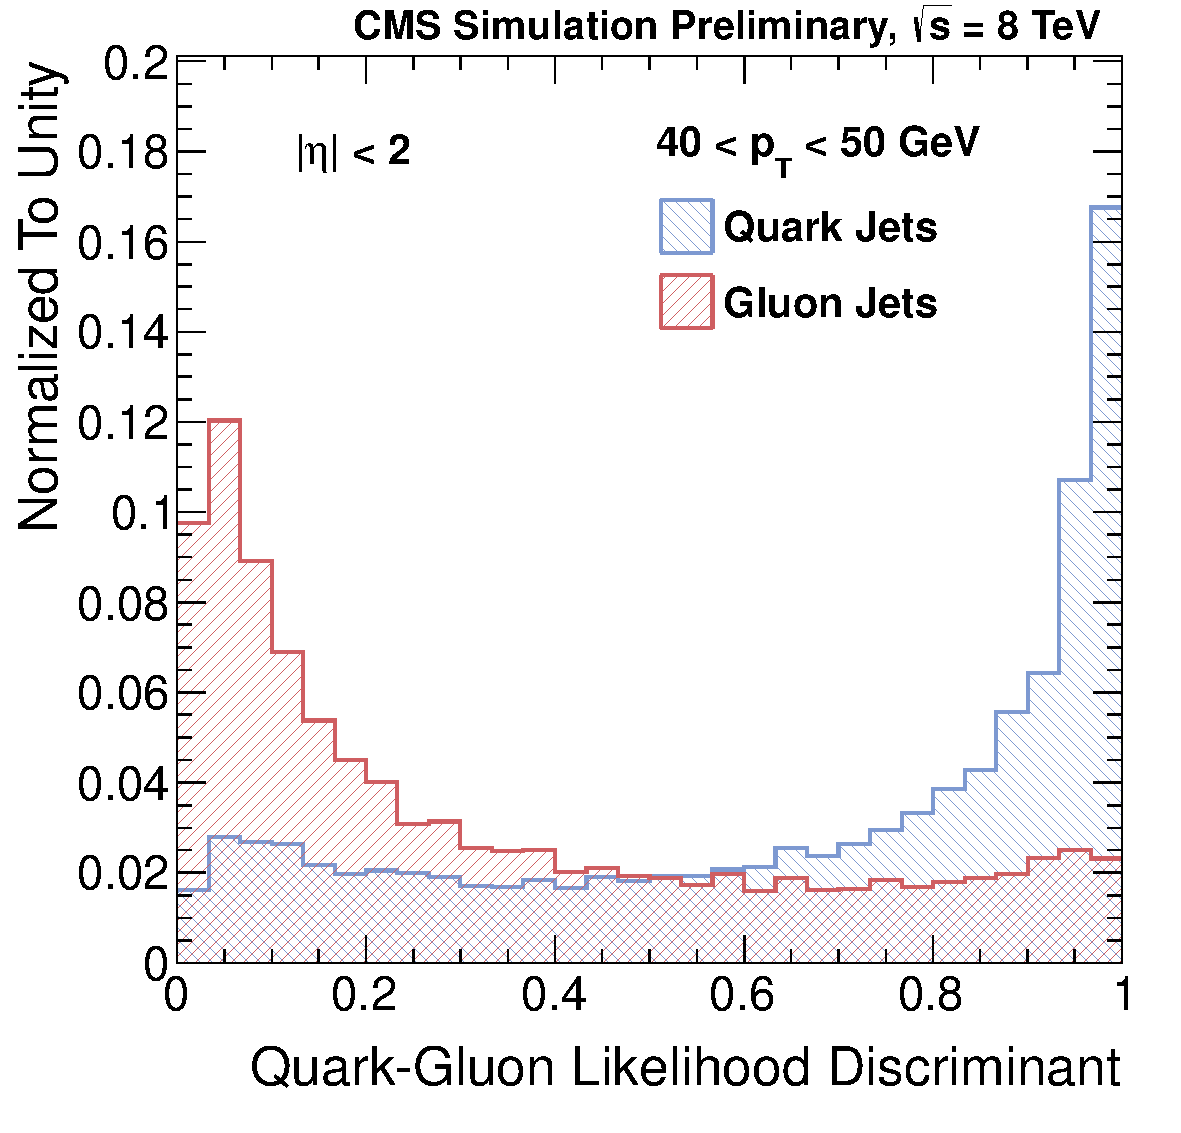
\includegraphics[width=.4\textwidth]{\PhDthesisdir/contents/chapter-JERC/reconstruction_des_jets/qgl.pdf}
\caption{Densité de probabilité de la fonction de vraisemblance utilisée pour discriminer les jets issus de gluons de ceux issus de quarks~\cite{CMS-PAS-JME-13-002}. En rouge, pour les jets issus de gluons. En bleu, pour des jets issus de quarks.}
\label{fig-chapter-JERC-section-jets_reco-subsec-flavor-qgl_likelihood}
\end{figure}
%Sirunyan_heavy_flavor_jets_2018 53
%Cacciari_pu_sub_jet_area_2008 54
%Sarle1994NeuralNA 55
%keras 57
%tensorflow 58
%\emph{The efficiency for the tagging of b jets and the mistagging rate for light-flavour jets has been measured in both data and simulation. The efficiency and mistagging rate of the simulation is corrected through the application of efficiency and mistagging scale factors. The values of these factors and a description of the methods used to determine them can be found in Ref.~\cite{Sirunyan_heavy_flavor_jets_2018}.}
